\documentclass[11pt]{article}
\usepackage{geometry}                
\geometry{letterpaper}                   

\usepackage{listings}
\usepackage{color}
\usepackage{graphicx}
\usepackage{epstopdf}
\usepackage{varioref}
\usepackage[numbers]{natbib}
\usepackage[squaren]{SIunits}
\usepackage{amssymb, amsmath}

\DeclareGraphicsRule{.tif}{png}{.png}{`convert #1 `dirname #1`/`basename #1 .tif`.png}

\title{Modelling Situations of Evacuation in a Multi-level Building}
\author{Hans Hardmeier, Andrin Jenal, Beat K\"ung & Felix Thaler}
\date{date} 

\begin{document}



\thispagestyle{empty}

\begin{center}

\includegraphics[width=5cm]{ETHlogo.eps}

\bigskip


\bigskip


\bigskip


\LARGE{ 	Lecture with Computer Exercises:\\ }
\LARGE{ Modelling and Simulating Social Systems with MATLAB\\}

\bigskip

\bigskip

\small{Project Report}\\

\bigskip

\bigskip

\bigskip

\bigskip


\begin{tabular}{|c|}
\hline
\\
\textbf{\LARGE{Insert Title Here}}\\
\textbf{\LARGE{...}}\\
\\
\hline
\end{tabular}
\bigskip

\bigskip

\bigskip

\LARGE{Name 1 \& Name 2}



\bigskip

\bigskip

\bigskip

\bigskip

\bigskip

\bigskip

\bigskip

\bigskip

Zurich\\
March 2012\\

\end{center}



\newpage

%%%%%%%%%%%%%%%%%%%%%%%%%%%%%%%%%%%%%%%%%%%%%%%%%

\newpage
\section*{Agreement for free-download}
\bigskip


\bigskip


\large We hereby agree to make our source code for this project freely available for download from the web pages of the SOMS chair. Furthermore, we assure that all source code is written by ourselves and is not violating any copyright restrictions.

\begin{center}

\bigskip
\bigskip
\bigskip
\bigskip


\begin{tabular}{@{}p{3.3cm}@{}p{6cm}@{}@{}p{6cm}@{}}

\begin{minipage}{3cm}

\end{minipage}
&
\begin{minipage}{6cm}
\vspace{2mm} \large Hans Hardmeier

 \vspace{\baselineskip}

\end{minipage}
&
\begin{minipage}{6cm}

\large Andrin Jenal

\end{minipage}

\end{tabular}

\bigskip
\bigskip
\bigskip
\bigskip


\begin{tabular}{@{}p{3.3cm}@{}p{6cm}@{}@{}p{6cm}@{}}

\begin{minipage}{3cm}

\end{minipage}
&
\begin{minipage}{6cm}
\vspace{2mm} \large Beat K\"ung

 \vspace{\baselineskip}

\end{minipage}
&
\begin{minipage}{6cm}

\large Felix Thaler

\end{minipage}
\end{tabular}

\end{center}
\newpage

%%%%%%%%%%%%%%%%%%%%%%%%%%%%%%%%%%%%%%%




\includegraphics[width=\textwidth]{declaration_of_originality.jpg}

% you MUST include the ETH declaration of originality here; it is available for download on the course website or at http://www.ethz.ch/faculty/exams/plagiarism/index_EN; it can be printed as pdf and should be filled out in handwriting

\newpage

%%%%%%%%%% Table of content %%%%%%%%%%%%%%%%%

\tableofcontents

\newpage

%%%%%%%%%%%%%%%%%%%%%%%%%%%%%%%%%%%%%%%



\section{Abstract}

If you are an ETH-Student, you know that at lunch time it is almost impossible 
to go out of the building through the main entrance to the polyterasse, because
of the number of students trying to leave at the same time. What would happen,
if in addition to that, an evacuation was involved? Have you ever imagined, how
an evacuation at the ETH Main building, ETH CAB-Building or even at your own home
would look like? How many people would be able to leave simultaneously? What is the
best strategy for people to leave? How would the perfect evacuation plan for your
school or enterprise building look like?

In this work, we decided to elaborate a program that is flexible enough to
calculate the fastest exit for every given building structure. Using a "2D Range
Tree Datastructure" to solve this complex problem and to improve the access to
the forces over each agent, the program is capable of simulating the
evacuation efficiently.

Different from all other similar projects, we also focused on an efficient and
realistic implementation of the program. For the preprocessing, the "\textit{Fast
Sweeping} Algorithm Method" 
enabled us to have only some seconds of initialization time (instead of some
minutes with "\textit{Fast Marching} Algorithm" (See \ref{implementation}).
Using our own "2D Range Tree" data structure to handle the numerous amount of
agents enables us to simulate large buildings with many agents and with a
realistic force model.

\section{Individual contributions}

We all worked together in this project and used the individual strengths of each
of us to achieve the best possible result. Detailed information about the
individual contribution can be obtained from the git history.

Carl Hans Peter Hardmeier Samame, alias Hans Hardmeier, was 
responsible for some parts of the documentation, verification of the
\textit{MATLAB}-code and calculating efficiency using different operating
systems (i.e. Mac OS 10.6).

Contributing to some core functionalities of the social force model, especially repulsive effects,
Andrin Jenal focused on the modeling of the buildings layout used in the simulation.
Additionally, he elaborated some sections of the documentation.

Beat K\"ung did most of the plotting functionality and the definition \&
implementation of the configuration and building image file. He also did several
sections of the documentation.

Felix Thaler implemented the algorithms written in \textit{C}, using \textit{MATLAB}'s \textit{MEX}-interface.
These are efficient \textit{Fast Sweeping}, a 2D \textit{Range Tree} and fast bilinear interpolation.
Further he developed the basic simulation framework and added the social force model as well as some
custom algorithms, for instance one to minimize wall penetration of agents. Some sections of the documentation are
written by him, too.


\section{Introduction and Motivations}

\subsection{Introduction}

Simulating the evacuation scenario of a single-level building is well known but
is not general enough. Though we want to introduce a more sophisticated
simulation within a multi-level building. E.g.: What would happen, if a
multi-level building has to be evacuated? Which escape routes would be mostly
used? Which effects would the pressure of other persons have to the
situation? Since tower buildings are getting more common in large cities,
engineers have to care more about the behavior in situations of emergency,
namely evacuations. Apart of the mathematical model and implementation for
solving this problem, we also wanted to increase the utility of this program for
all readers by giving the possibility of calculate different scenarios in
different buildings given by the user. In this work, we will mostly work with
the map of the ETH building, however, there are more configurations in the data
folder and one can replace any map with others that meet the properties of the
Figure \ref{building floor image} in section \ref{matlab code}.

\subsection{Motivation}

Intuitive expectations and mathematical model results can stay sometimes in
contradiction. Our intuition is full of little concepts that are hard to realize
in a conscient way.  Using the language of mathematics, we want to describe
formaly all the elements that contribute to the complex result of the human
behavior. However, a common point of motivation within the group is the
connection between the 'real' World and the mathematical formalism.

On the other side, we, as ETH-Students, are not sure if the evacuation potential
(the property of a buiding of being evacuated efficiently) of our ETH-buildings
are enough for the amount of students during a normal week day. We also want to
help the people around the world that have a similar question to find an answer.
This two points gave us the ideas and motivation to create a flexible tool that
simulates a real-world scenario for any given building or even structure (i.e.
planes or boats).


\subsection{Fundamental Questions}

In the first place, we all are wondering \textit{how exaclty an implementation
of a social force model looks like}, based on already published papers coping
with this problem \cite{SFMPD} \cite{SDFEP}. Of special interest is also
\textit{how this model can be implemented efficiently for a multilevel building
and how it can be extended to add some dynamic features}. Moreover we are keen
to understand \textit{how the simulation behaves applying the model to a real
building like the ETH main building}. Generally speaking, \textit{how realistic
is the behavior of the agents used in our model?}.

\section{Description of the Model}
\subsection{General Model}

For our model, we will create a relatively general framework for behavioral
simulation in evacuation scenarios based on the social force model introduced by Dirk Helbing \cite{SDFEP}.
A core investigation is a simulation, beginning in a general everyday situation,
where people are spread randomly in their office or somewhere in the hallway and ending in an evacuation scenario.
At the end we should be able to make strong
statements anwsering our fundamental questions.
Based on the forces explained in the following paragraphs, we tried to figure
out how agents overcome major obstacles like tiny passages, stairs or pillars.

\subsection {Forces}

We implemented the model's forces as described in \cite{SDFEP}, a brief overview is given here.

The reactions of the agents will mainly be influenced by different forces, modelparameters and the building structure itself.
Describing this problem in mathematical terms, leads to an equation, where the mass, the desired direction $f_{D}$, the repulsive forces $f_{ij}$ and the wall force $f_{iW}$ of each individual agent contribute to the change of velocity in time.\\
Helbing stated this problem as the following:"We assume a mixture of socio-psychological and physical forces influencing the behavior in a crowd: each of $N$ pedestrians $i$ of mass $m_{i}$ likes to move with a certain desired speed $v_{i}^0$ in a certain direction $\mathbf{e}_{i}^0$, and therefore tends to correspondingly adapt his or her actual velocity $\mathbf{v}_i$ with a certain characteristic time $\tau_{i}$. Simulataneously, he or she tries to keep a velocity-dependent distance from other pedestrians $j$ and walls $W$."

\begin{equation}
m_{i}\frac{\mathsf{d}\mathbf{v}_{i}}{\mathsf{d}t}=m_{i}f_{D}+\sum \limits_{j(\neq{i})}{f_{ij}}+\sum \limits_{W}{f_{iW}}
\end{equation}

That means the change of position $\mathbf{r}$ is given by the velocity: $\mathbf{v}_{i}=\frac{\mathsf{d}\mathbf{r}_{i}}{\mathsf{d}t}$\\
To understand the different parties, they will be explained briefly.

\subsubsection{Desired Direction Force}

An agent always has a desired direction $e(t)$ in which he wants to walk currently with a desired speed of $v(t)$. 
The reaction time $\tau$ affect the speed of the directional change.

\begin{equation}
f_{D}=\frac{v_{i}^{0}(t)\mathbf{e}_{i}^{0}(t)-\mathbf{v}_{i}(t)}{\tau_{i}}
\end{equation}

\subsubsection{Repulsive Interaction Force}

As people don't like to get too close to each other, the main component of this
formula is a rather psychological aspect and plays an important role to keep
agents apart from each other. However if it should happen that agents get too
close, two additional forces, the 'body force' counteracting body compression
and 'sliding friction force' contribute to the repulsive force to ensure a
certain distance. \cite{SDFEP} 

\begin{equation}
f_{ij}=\left\{A_{i}exp[(r_{ij}-d_{ij})/B_{i}]+kg(r_{ij}-d_{ij})\right\}\mathbf{n}_{ij}+\kappa g(r_{ij}-d_{ij})\triangle v_{ji}^t\mathbf{t}_{ij}
\end{equation}

According to Helbing the repulsive interaction force $A_{i}exp[(r_{ij}-d_{ij})/B_{i}]\mathbf{n}_{ij}$ describes the psychological tendency of two pedestrians $i$ and $j$ to stay away from each other, where $A_i$ and $B_i$ are constants. 
"$d_{ij}=\|r_i-r_j\|$ denotes the distance between the pedestrians' centres of mass, and $\mathbf{n}_{ij}=(n_{ij}^1, n_{ij}^2)=\mathbf{r_i}-\mathbf{r_j}/d_{ij}$ is the normalized vector pointing from pedestrian $j$ to $i$.
The pedestrians touch each other if their distance $d_{ij}$ is smaller than the sum $r_{ij}=(r_i+r_j)$ of their radii $r_i$ and $r_j$."\cite{SDFEP}
If this is the case two addtional forces are considered:
$k(r_{ij}-d_{ij})\mathbf{n}_{ij}$ and $\kappa(r_{ij}-d_{ij})\triangle
v_{ij}^t\mathbf{t}_{ij}$. "Here $\mathbf{t}_{ij}=(-n_{ij}^2,n_{ij}^1)$ means
the tangential direction and $\triangle
v_{ij}^t=(\mathbf{v}_j-\mathbf{v}_i)\cdot\mathbf{t}_{ij}$ and the function
$g(x)$ is zero if the pedestrians do not touch each other $(d_{ij}>r_{ij})$,
and otherwise equal to the argument $x$."\cite{SDFEP}

\subsubsection{Wall Force}
Similar to the repulsive interaction force people don't want to get too close to walls neither. To prevent this, the wall force is introduced.
Helbing states it the following:"$d_{iW}$ means the distance to wall $W$, $\mathbf{n}_{iW}$ denotes  the direction perpendicular to it, and $\mathbf{n}_{iW}$ the direction tangential to it, the corresponding interaction force with the wall is given by:" \cite{SFMPD}

\begin{equation}
f_{iW}=\left\{A_{i}exp[(r_{i}-d_{iW})/B_{i}]+kg(r_{i}-d_{iW})\right\}\mathbf{n}_{iW}-\kappa g(r_{i}-d_{iW})(\mathbf{v}_{i}\cdot\mathbf{t}_{iW})\mathbf{t}_{iW}
\end{equation}

\section{Implementation}\label{implementation}
Our goal was a fast implementation of the model. So we decided to use the
\textit{Fast Sweeping} algorithm instead of the \textit{Fast Marching} alorithm
to calculate the fastest way out of a building. We knew that \textit{MATLAB}
code is not very fast and \textit{MATLAB} provides an interface for other
programming languages. So we used the \textit{C} programming language to
implement the \textit{Fast Sweeping} method.

Later in the development process we discovered another bottleneck in our code:
The social force between the agents which runs in $ O(n^2) $. Felix Thaler then
introduced a \textit{Range Tree} for this problem, which he also implemented in
\textit{C}.


\subsection{\textit{MATLAB} Code} \label{matlab code}
We wanted to create a flexibel model which can be used to simulate many
possible building structures.
Each scenario is described in a configuration file. This includes for example how many
agents are placed on each floor or the timestep of the simulation (the exact
definition can be found in the file \verb+data/config_file_structure+). Each config
file also references one or more building floor images.
Figure \vref{building floor image} describes how a building floor
image must look like. The agents are placed randomly within the agents spawning
area(s).

\begin{figure}[ht]
\centering
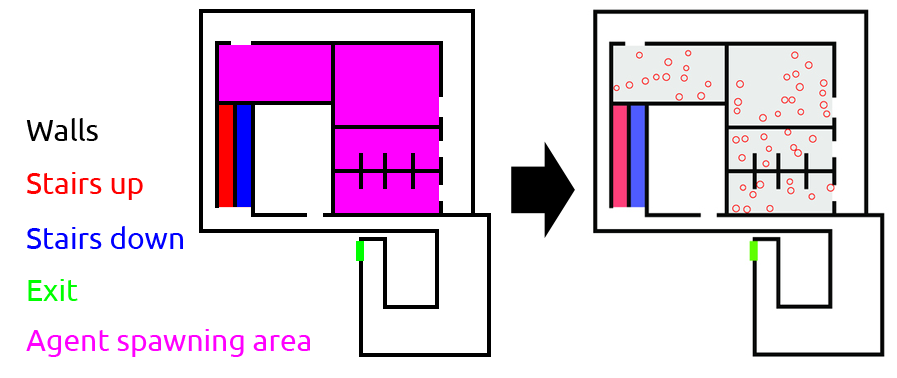
\includegraphics[width=\textwidth]{./images/config_floor_description.png}
\caption{Left the building floor image and right how it looks when the
simulation is running} 
\label{building floor image}
\end{figure}

Since \textit{MATLAB} is not really object-oriented, we used a big data
structure (called \verb+data+) that includes all internal data that we use (eg.
the floors and agents).  It is passed as an argument for every function that
needs it.

\subsection{Pathfinding}
As described in \cite{SFMPD}, the agents always try to reach their desired destination
using the shortest possible path. As we use raster graphics to encode simulation data,
we decided to use the same discrete grid to compute the nearest path to an exit for every point approximately.
Mathematically, this can be expressed as an partial differential equation, the 2D Eikonal equation (equation \ref{eq:eikonal}).

\begin{equation} \label{eq:eikonal}
\|\mathbf{\nabla} d(\mathbf{x})\|=1 \quad d:\!\mathbb{R}^{2}\to\mathbb{R},\mathbf{x}\in\mathbb{R}^{2}
\end{equation}

The solution $d(\mathbf{x})$ now gives the distance to the nearest exit point, its
negative gradient $-\mathbf{\nabla}d(\mathbf{x})$ therefor always points in the 
direction of the shortest path towards the desired exit. There are mainly two
competitive agorithms for solving this equation efficiently. First there is the
\textit{Fast Marching} method, a specialized version of Dijkstra's well known 
algorithm \cite{dijkstra59a}. The alternative is \textit{Fast Sweeping}, which 
leads to a much simpler implementation, faster calculation and better algorithmic
complexity of $O(n)$ instead of $O(n\log n)$ with respect to the discretization size.
We therefor implemented an efficient \textit{Fast Sweeping} method, closly following
\cite{Zhao04afast} as a basis of our pathfinding and repulsive wall forces. The 
algorithm uses an upwind finite difference scheme where our mesh is defined by 
the input images. The implementation was done \textit{C} and not directly in
\textit{MATLAB}, using optimized boundary condition handling for our pruposes.
Our benchmarks showed a high speed increase compared to other Eikonal solvers,
e.g. the "Accurate Fast Marching" implementation as found at \textit{MATLAB CENTRAL}
\cite{fastmarching}.


\subsection{Profiling \& Optimization}


Using the \textit{Profiler}-function of \textit{MATLAB}, we were able to discuss
the efficiency of our implementation. The image \vref{cab profile} shows the
time consumption for the calculation of the evacuation of 2 floors (ETH
CAB-Building Floors E and F) within 4087 seconds.

The first version of our simulation showed a different profiling behavior: The
functions \verb+interp2+ and \verb+addAgentRepulsiveForce+ were at the top and
thus needed most of the calculation time. Now, after our improvements, they are
further down in the profiling ranking, meaning they are more efficient. These
improvements decreased the time for simulation significantly.

\begin{figure}[ht]
\centering
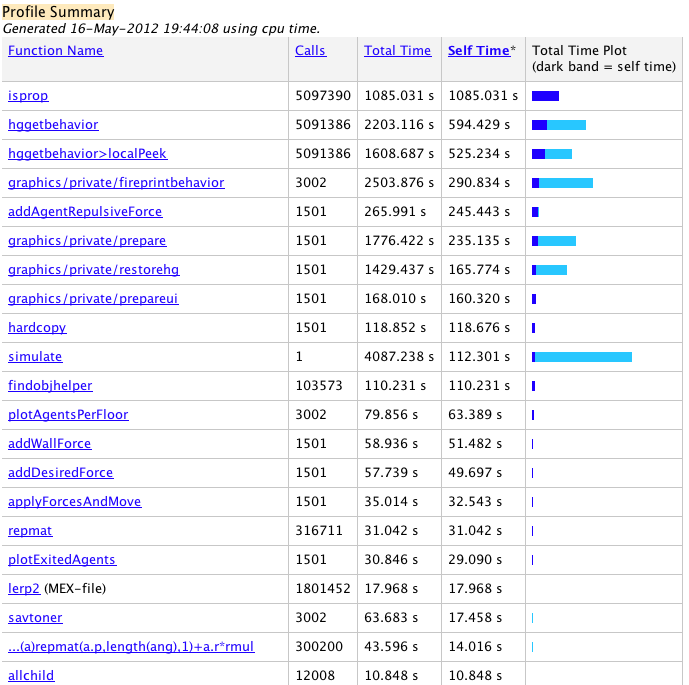
\includegraphics[width=0.8\textwidth]{./images/profiler.png}
\caption{Profile of the calculation for the CAB-Building with 300 agents over 3 different floors} 
\label{cab profile}
\end{figure}

\subsubsection{Parallelization}

We tried to optimize the code using the parallel for-loop \verb+parfor+ in
\textit{MATLAB}. In the function \verb+applyForcesAndMove+ we replaced the
for-loop over the agents with \verb+parfor+. We measured the time using an input
with 200 agents on a 4 core machine using 5 \textit{MATLAB} workers. The result
was that the parfor version was even slightly slower than the serial version.
The reason for this is how \textit{MATLAB} implements \verb+parfor+: all the
memory that is used by a worker must be sent to this worker.  Each agent must
access the building floor image randomly and this creates a large amount of
memory that must be transferred to each worker, which leads to a decreasing
performance.  This is why we decided not to use \verb+parfor+ or any other
parallelization in our implementation.

\subsubsection{Replacing \textit{MATLAB} standard functions}

Through our first messures, we realised that the function \verb+interp2+
consumed a lot of resources and time. We decided to create our own operator
called \verb+lerp2+ (written in \textit{C}) that interpolates between data points. It finds values of a
two-dimensional function interpolating the data at intermediate points bilinearly.
Here the different given data points are the current values of the frame $i-1$
for the frame $i$. 

\subsubsection{Range Tree}
The most time consuming part in our program is the calculation of the interaction
forces between the agents, at least if their count is high enough. To reduce the
natural complexity of order $O(n^{2})$ of this inter-agent interaction, we can clamp forces
with little effect, e.g. in our implementation all forces smaller than $ 10^{-4}\newton$.
As they are exponentially decreasing, the distance in which the forces need to be adressed
is only several meters, so a big part of them can just be ignored without introducing 
a significant error.

To get all agents influenced by another agent by a force bigger than a threshold, we need to be able
to search neighbours of any agent within a given distance. To efficiently query 
these agents, we implemented a 2D \textit{Range Tree} in \textit{C}, which allows query times
of order $O(\log^{2} n+k)$, where $n$ is the total number of agents and $k$ is the number of
queried agents \cite{algdat}. In larger simulations this reduces simulation times by a significant factor.

\section{Simulation Results and Discussion}

\subsection{Expected Results}

We expect the stairs and the main building exit to be the bottlenecks. The
amount of people in lower levels is increasing with time until a certain point,
when most of the people have exited the building. Also we think that if the 
velocity of the people is higher, jams at the exit will increase.


\subsection{Simulation Results}

We tested our algorithm mainly by simulating an evacuation of ETH's CAB building.
The floor plans were downloaded from \cite{ethfloors} and converted to our coded bitmap representation.
The results of the simulation are, as expected, comparable to those of Helbing as described in \cite{SFMPD} and \cite{SDFEP}.
Our implementation realisticly shows some bottlenecks which get heavily crowded soon, especially the regions before stairs and exits.
The speed of the agents decreases heavily due to the crowd and the time they need to reach the exits therefor increases rapidly.
As we used real world units in our model, it was relatively simple to get the right scale for the simulation,
nonetheless we found that some agents got stuck at the doors, as they block each other.
This is of course not a very realistic behavior but due to the simplicity of our agents demand to reach the
exit with shortest Euklidean distance. It would be interesting to use a more intelligent and natural search 
algorithm to determine the best path to escape, but this is out of the scope of this project, 
see also section \ref{subsection:Improvements} about other possible improvements.

\begin{figure}[ht]
\centering
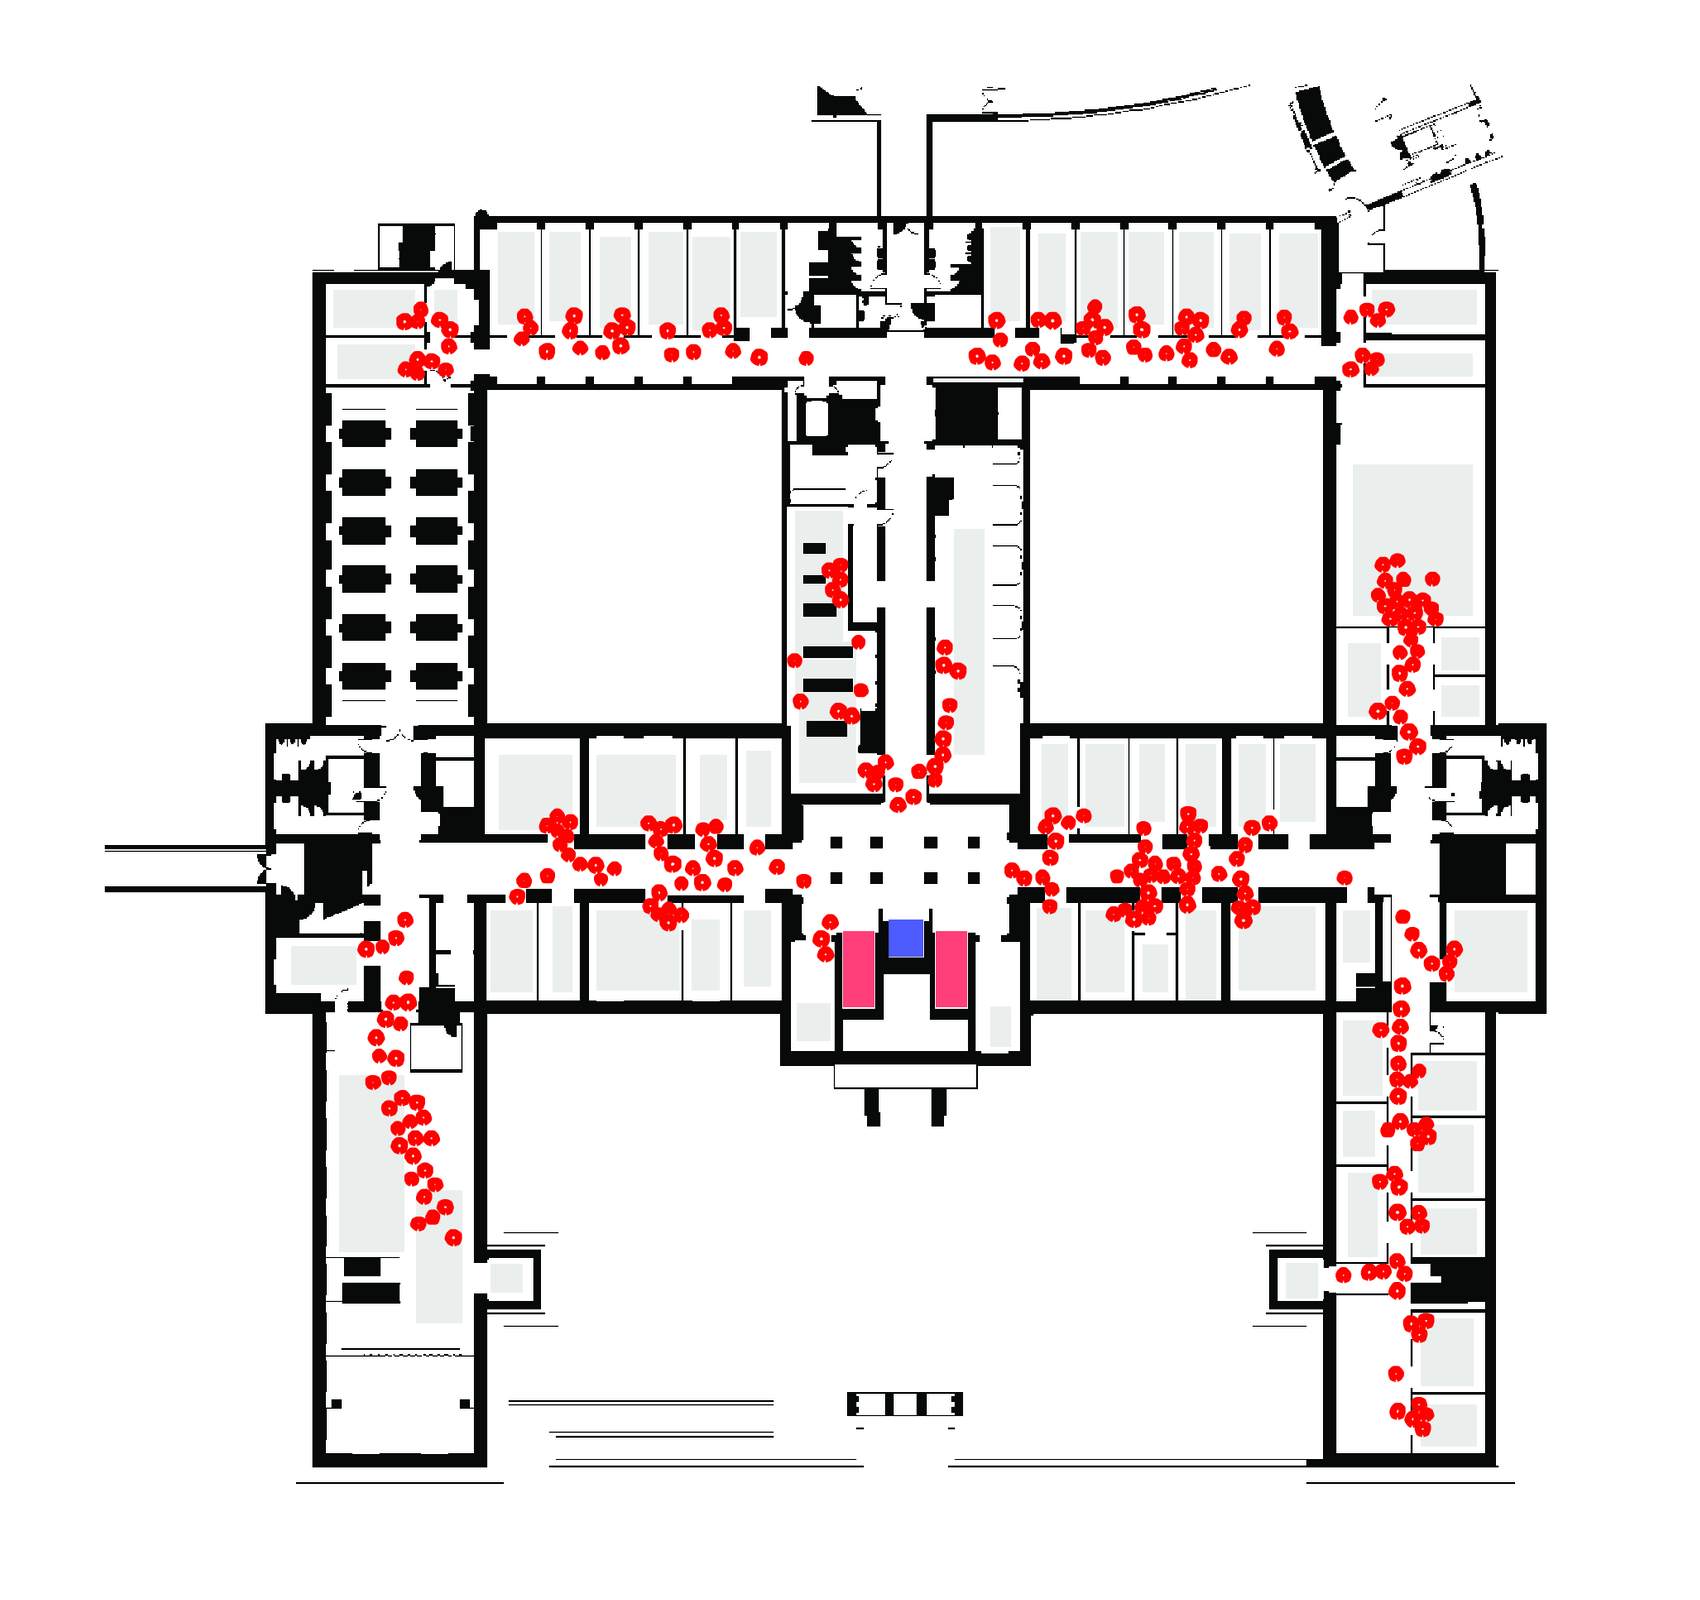
\includegraphics[width=0.8\textwidth]{./images/cab1.png}
\caption{Visualisation of evacuation in the CAB Building E Floor} 
\label{cab1}
\end{figure}

\subsubsection{Comparison to previous projects}

As there were already other projects in this course which studied agent based evacuation simulations, 
we decided to compare our results to those of an older project, namely the project 
"Evacuation Bottleneck: Simulation and analysis of an evacuation of a high-school building with \textit{MATLAB}"by
Alexander J\"ohl and Tom\'{a}\v{s} Nyitray \cite{oldproj}.

They use a very simplicistic model, incorporating just two forces: 
one pointing towards the nearest exit and one inter-agent force. The former is comparable to the one used in our model, but missing some
sophisticated interpolation on the discretized grid, while the latter is following a much simpler approach 
and is just a force centered around the agents with inverse linear fall-off.
As their inter-agent forces are so weak, the stability timestep restriction is not that tight and therefor the simulation times are very low.
In our implementation using the forces as defined in \cite{SDFEP} one the other hand, 
there is a much stricter timestep restriction, leading to higher simulation times to guarantee stability, but in this case still lower than 5 minutes.
But a linear force can't simulate realistic interaction between the agents and they can
easily penetrate each other. Therefor it is impossible to simulate crowding and evacuation bottlenecks.

Further, their floorplan is significantly less detailed than our implementation allows and no proper scaling seems
to be mentioned or implemented, this made it difficult to get similar parameters, especially because in our 
model the collision detection works accurately using the agents radii, which means they get stuck at narrow doors.

To recreate the speed of their agents, a time lapse simulation seemed to be most appropriate and indeed, we could get some similar 
results. Nonetheless our model does not show the weaknesses described above, there are no overlapping agents and they walk along straight lines.

\begin{figure}[ht]
\centering
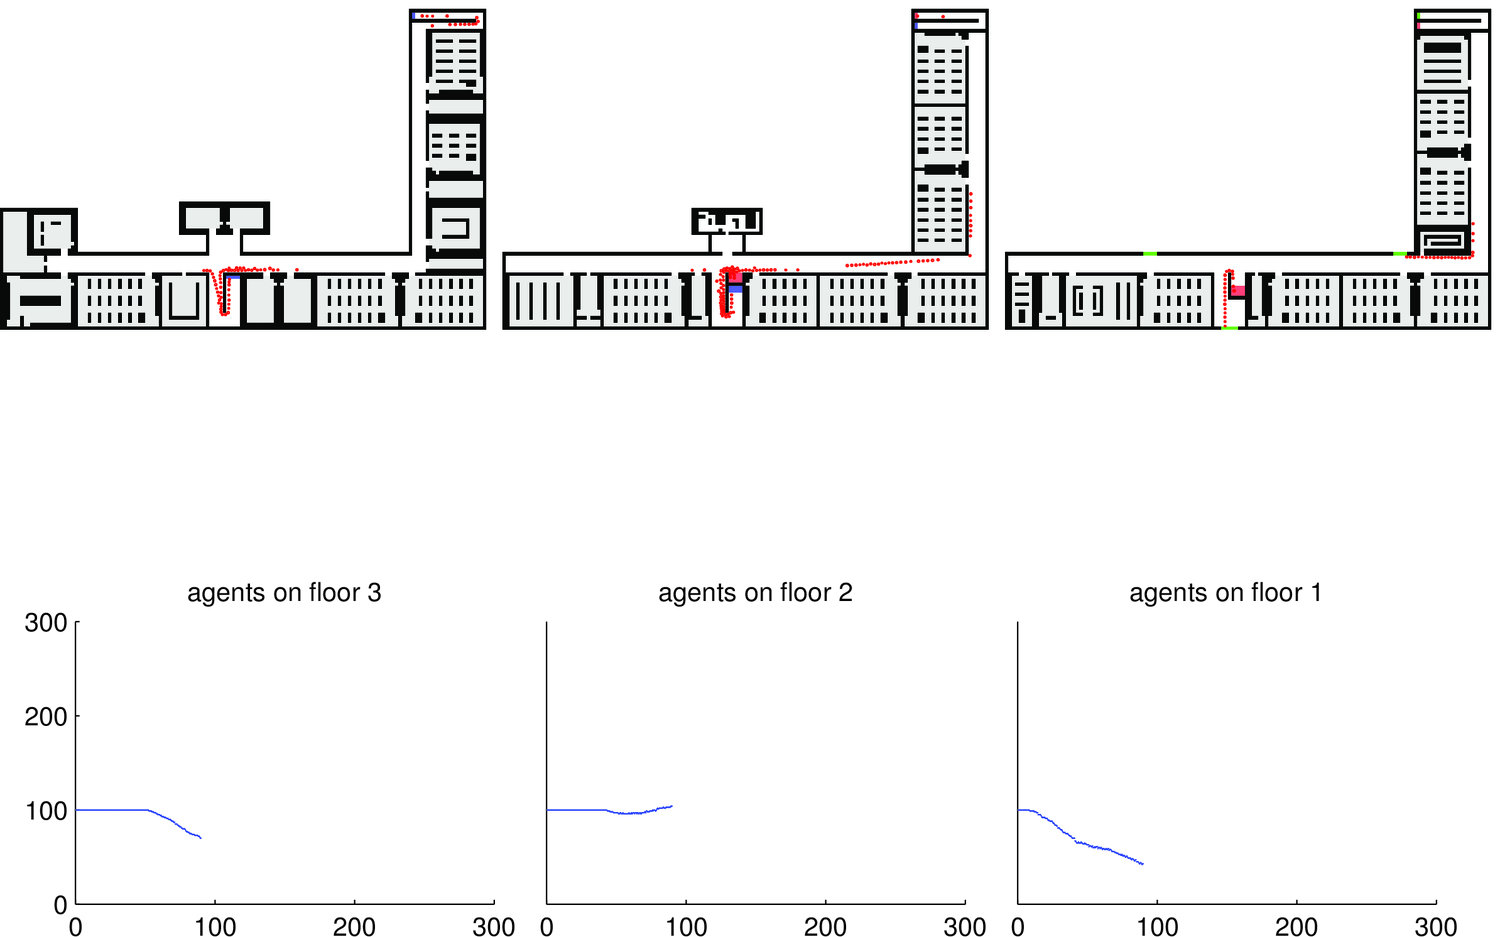
\includegraphics[width=0.8\textwidth]{./images/swsl.png}
\caption{One frame of our simulation of the building given in \cite{oldproj}.} 
\label{swsl}
\end{figure}

\subsection{Improvements} \label{subsection:Improvements}
There are several things that could be done to further improve our social force
model and to reduce the calculation time used to simulate.

\begin{description}
	\item[choice of exit] Our simulation of the CAB building shows that most of
		the agents take the side exit on the lowest floor, and only a few exit
		through the main door, which is right beside the side exit. This is not
		very realistic and could be improved by adding intelligence to the
		agents. For example each agent could decide which exit he/she wants to
		take, and also consider jams at the visible exits.
	\item[panic factor] We did not implement the panic factor mentioned in
		\cite{SDFEP}. In reality, people in panic behave less organized, they
		probably don't always run towards the nearest exit.
	\item[timestep] If the timestep in the config file is too big, the
		simulation becomes unstable and behaves like a billiards game. This
		sometimes also happens when a lot of agents are crowded and push in one
		direction. Adaptive timestepping or an implicit integration scheme
		could be introduced to solve this issue.
	\item[agent velocity] All agents are currently equally fast, which is of
		course different from reality.
	\item[doors] In our simulations, the doors of the CAB building were
		sometimes too narrow for the agents to exit. But this issue can easily
		be resolved by changing the building map or the agent radii in the
		config file.
	\item[calculation time] For no obvious reason, the time used to calculate
		one simulation-step (one frame) increases linearly over time. We
		identified the plotting routine as the culprit, but we were not able
		to figure out whether this is a \textit{MATLAB} problem or our plotting
		calls are to blame for this. Certainly, a big performace advantage would
		be to write the whole simulation in \textit{C/C++}. 
\end{description}

\section{Summary}

Summarizing the results of the simulation for the purpose of answering the fundamental questions 
of this project, we can claim that the implementation of different force models
has not  been a major problem. Nonetheless the implementation
of an \textit{realistic} evacuation model is far more complicated than expected.
Details like individual-reactions or non-expected events have been 
ignored for the sake of simplicity, although they enjoy of a special importance
for this kind of social force models.

\textit{MATLAB} was powerful enough to simulate and it also provides a wide spectrum of useful features and functions.
Unfortunately, the efficience of them cannot be compared to their functional equal features in 
other programming languages like \textit{C or C++}. Nevertheless, \textit{MATLAB} is a good tool
for projects, which have not the intention of simulating a social force model in
real time.

\subsection{Thanks}

In this section we would like to thank the MSSSM-Group from the ETH in Zurich, Switzerland
directed by Karsten Donnay and Stefano Balietti for their engagement in the lecture
"Modeling and Simulating Social Systems with \textit{MATLAB}" during the Spring Semester 2012.

\section{References}

\begin{thebibliography} {9}
	
	\bibitem{Zhao04afast} Zhao, Hongkai (2004): A Fast Sweeping Method for Eikonal Equations.
	\bibitem{SFMPD} Helbing, Dirk; Molnar, Peter (1995): Social Force Model for Pedestrians Dynamics.
	\bibitem{AACIBF} Helbing, Dirk; Johnson, Anders (2006): Analytical Approach to Continuous and Intermittent Bottleneck Flows.
	\bibitem{ACPPD} Schadschneider, Andreas et al. (2002): CA Approach to Collective Phenomena in Pedestrian Dynamics.	
	\bibitem{DCD} Helbing, Dirk; Johansson, Anders (2007): Dynamics of crowd disasters: An empirical Study.
	\bibitem{SDFEP} Helbing, Dirk et al. (2000): Simulating dynamical features of escape panic.
	\bibitem{SPCD} Helbing, Dirk et al. (2005): Self-Organized Pedestrian Crowd Dynamics: Experiments, Simulations, and Design Solutions.
	\bibitem{dijkstra59a} Dijkstra, Edsger W. (1959): A Note on Two Problems in Connexion with Graphs.
	\bibitem{fastmarching} Kroon, Dirk-Jan (2011): http://www.mathworks.com/matlabcentral/fileexchange/24531-accurate-fast-marching
	\bibitem{algdat} Ottmann, Thomas; Widmayer, Peter (2002): Algorithmen und Datenstrukturen, 4. Auflage.
	\bibitem{ethfloors} ETH Zürich, Version 2011.1 prod (prod red2): http://www.rauminfo.ethz.ch
	\bibitem{oldproj} Jöhl, Alexander; Nyitray Tom\'{a}\v{s}: Evacuation Bottleneck: Simulation and analysis of an evacuation of a high-school building with \textit{MATLAB}, https://github.com/jjoolloo/Swiss-Slovak-misunderstanding

\end{thebibliography}

% use \cite{SFMPD} for citation

\section{Appendix}

\subsection{Code}

% define colors
\definecolor{commentcolor}{RGB}{89, 168, 89}
\definecolor{keywordcolor}{RGB}{68, 68, 255}
\definecolor{stringcolor}{RGB}{205, 139, 247}
\definecolor{numbercolor}{RGB}{128, 128, 128}
\definecolor{bgcolor}{RGB}{245, 248, 253}

% define listings style
\lstset{
  language=Matlab,
  basicstyle=\footnotesize\ttfamily,
  numbers=left,
  numberstyle=\tiny\color{numbercolor},
  stepnumber=2,
  numbersep=5pt,
  backgroundcolor=\color{bgcolor},
  showspaces=false, 
  showstringspaces=false,
  showtabs=false,
  frame=lines,
  rulecolor=\color{black},
  tabsize=2,
  captionpos=b,
  breaklines=true,
  breakatwhitespace=true,
  title=\lstname,
  commentstyle=\color{commentcolor},
  keywordstyle=\color{keywordcolor},
  stringstyle=\color{stringcolor}
}

\subsubsection{\textit{MATLAB} code}

% code is ordered alphabetically by file name...

\lstinputlisting[caption=addAgentRepulsiveForce.m]{../code/addAgentRepulsiveForce.m}
\lstinputlisting[caption=addDesiredForce.m]{../code/addDesiredForce.m}
\lstinputlisting[caption=addWallForce.m]{../code/addWallForce.m}
\lstinputlisting[caption=applyForcesAndMove.m]{../code/applyForcesAndMove.m}
\lstinputlisting[caption=checkForIntersection.m]{../code/checkForIntersection.m}
\lstinputlisting[caption=compileC.m]{../code/compileC.m}
\lstinputlisting[caption=initAgents.m]{../code/initAgents.m}
\lstinputlisting[caption=initEscapeRoutes.m]{../code/initEscapeRoutes.m}
\lstinputlisting[caption=initialize.m]{../code/initialize.m}
\lstinputlisting[caption=initWallForces.m]{../code/initWallForces.m}
\lstinputlisting[caption=loadConfig.m]{../code/loadConfig.m}
\lstinputlisting[caption=plotAgentsPerFloor.m]{../code/plotAgentsPerFloor.m}
\lstinputlisting[caption=plotExitedAgents.m]{../code/plotExitedAgents.m}
\lstinputlisting[caption=plotFloor.m]{../code/plotFloor.m}
\lstinputlisting[caption=simulate.m]{../code/simulate.m}

\subsubsection{\textit{C} code}

\lstinputlisting[language=C,caption=createRangeTree.c]{../code/createRangeTree.c}
\lstinputlisting[language=C,caption=fastSweeping.c]{../code/fastSweeping.c}
\lstinputlisting[language=C,caption=getNormalizedGradient.c]{../code/getNormalizedGradient.c}
\lstinputlisting[language=C,caption=lerp2.c]{../code/lerp2.c}
\lstinputlisting[language=C,caption=rangeQuery.c]{../code/rangeQuery.c}
\lstinputlisting[language=C,caption=tree.h]{../code/tree.h}
\lstinputlisting[language=C,caption=tree\_build.h]{../code/tree_build.h}
\lstinputlisting[language=C,caption=tree\_build.c]{../code/tree_build.c}
\lstinputlisting[language=C,caption=tree\_free.c]{../code/tree_free.c}
\lstinputlisting[language=C,caption=tree\_query.h]{../code/tree_query.h}
\lstinputlisting[language=C,caption=tree\_query.c]{../code/tree_query.c}
\lstinputlisting[language=C,caption=tree\_types.h]{../code/tree_types.h}



\end{document}  



 
